\documentclass{base}
% Dateikodierung ist utf8
\usepackage[utf8]{inputenc}
\usepackage{url}
\usepackage[export]{adjustbox}
\usepackage{amsmath}
\usepackage{listings}
\usepackage{tikz}
\usepackage{tabularx}
\usepackage{color,colortbl}
\usepackage{ulem}
\usepackage{pdfpages}
\usepackage{ wasysym }
\usepackage{ booktabs }
\usepackage{lscape}
\usepackage{multicol}
\usepackage{longtable}

\begin{document}

\Abgabeblatt{Assignment 6}{28.5.2018}{????}{????}{Yannis Rohloff (yannis@uni-bremen.de)}{Meng Liu(lium@uni-bremen.de)}{Islam Abushanab(is\_ab@uni-bremen.de)}

\lstset{
    language=Python,
    basicstyle=\ttfamily\small,
    aboveskip={1.0\baselineskip},
    belowskip={1.0\baselineskip},
    columns=fixed,
    extendedchars=true,
    breaklines=true,
    tabsize=4,
    prebreak=\raisebox{0ex}[0ex][0ex]{\ensuremath{\hookleftarrow}},
    frame=lines,
    showtabs=false,
    showspaces=false,
    showstringspaces=false,
    keywordstyle=\color[rgb]{0.627,0.126,0.941},
    commentstyle=\color[rgb]{0.133,0.545,0.133},
    stringstyle=\color[rgb]{01,0,0},
    numbers=left,
    numberstyle=\small,
    stepnumber=1,
    numbersep=10pt,
    captionpos=t,
    escapeinside={\%*}{*)}
}


\section*{Exercise 1:}

As we've seen earlier in the course we can encode circuits in cnf.
We can use this to encode our given problem.

First, we encode the circuit itself. The entire sorting network. with the input variables $x_0,\dots,x_5$ and the output variables $x'_0,\dots,x'_5$. Furthermore we have some intermediate variables that encode the inner nodes.
With this we can check if the network is satisfiable, which of course it is with our further constraints. Even for all possible partial valuations of $x_0,\dots,x_5$.

We add a negated version of the phase encoding, such that we search any possible solution of input variables that causes the output variables to be unsorted. If the formula then is satisfiable we know of at least one case which is sorted in the wrong order.

Our cnf would be built like this:
$$(\text{encoding of all circuits}) \land \neg (\text{phase encoding over variables } x'_0\text{ to } x'_5)$$
\begin{center}
	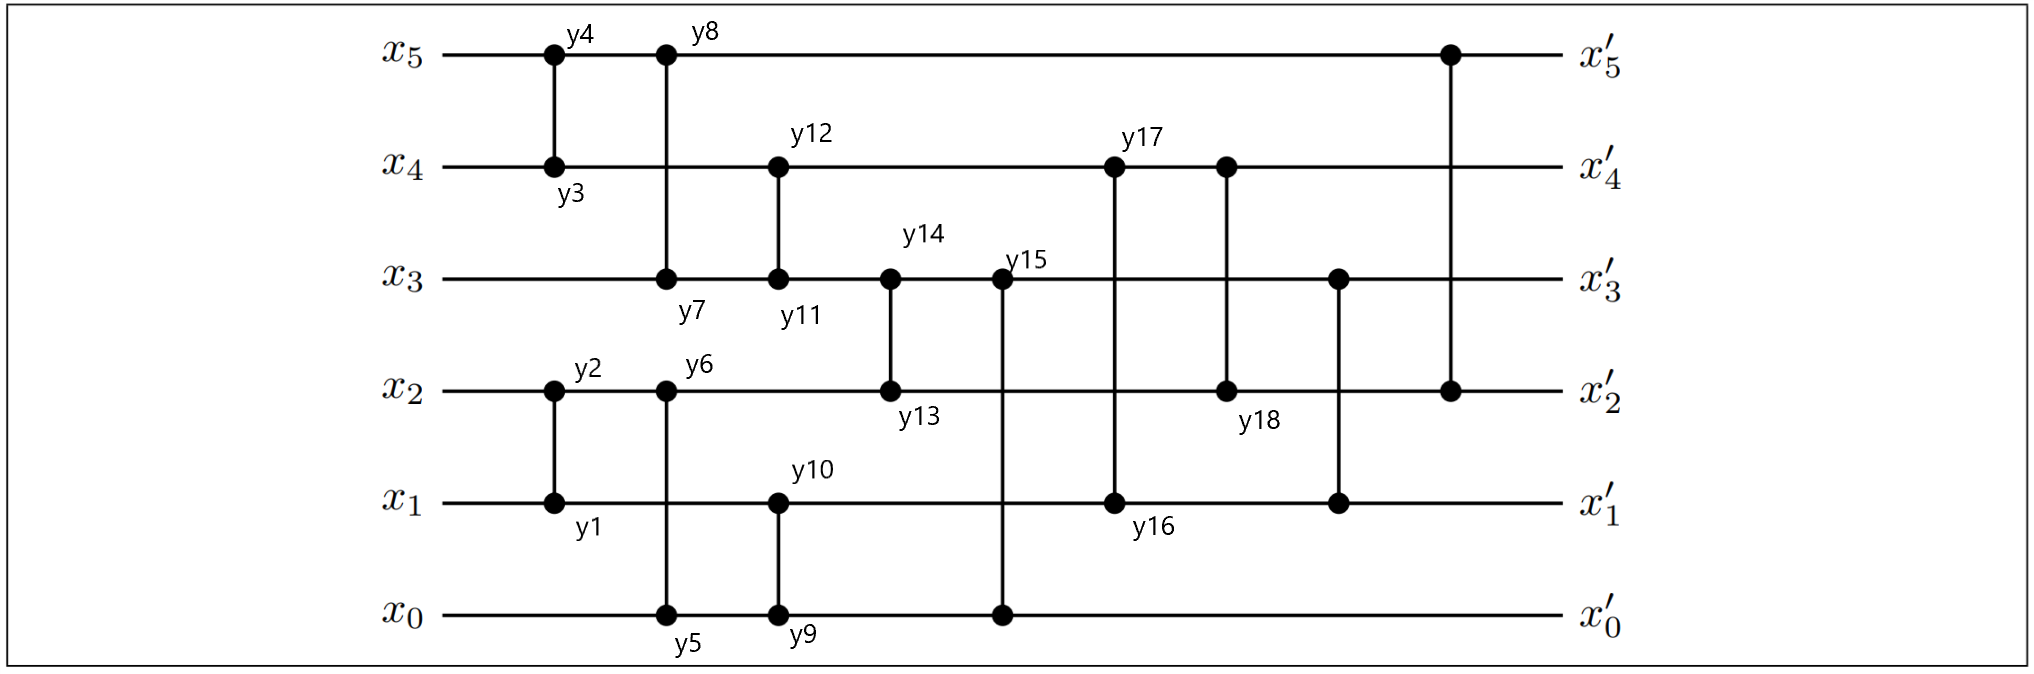
\includegraphics[width=\linewidth]{sorting_network.png}
	%\caption{Sorting network with variables}
\end{center}
SAT instance for encoding the circuits:
\begin{align*}
	%-1----------------------
	&\neg x_{1}\lor \neg x_{2}\lor y_{2} & x_{1}\lor \neg y_{2} && x_{2}\lor \neg y_{2}\\
	&x_{1}\lor x_{2}\lor \neg y_{1} & \neg x_{1} \lor y_{1} && \neg x_{2} \lor y_{1}\\
	%-3----------------------
	&\neg x_{4}\lor \neg x_{5}\lor y_{4} & x_{4}\lor \neg y_{4} && x_{5}\lor \neg y_{4}\\
	&x_{4}\lor x_{5}\lor \neg y_{3} & \neg x_{4} \lor y_{3} && \neg x_{5} \lor y_{3}\\
	%-5----------------------
	&\neg x_{0}\lor \neg y_{2}\lor y_{6} & x_{0}\lor \neg y_{6} && y_{2}\lor \neg y_{6}\\
	&x_{0}\lor y_{2}\lor \neg y_{5} & \neg x_{0} \lor y_{5} && \neg y_{2} \lor y_{5}\\
	%-7----------------------
	&\neg x_{3}\lor \neg y_{4}\lor y_{8} & x_{3}\lor \neg y_{8} && y_{4}\lor \neg y_{8}\\
	&x_{3}\lor y_{4}\lor \neg y_{7} & \neg x_{3} \lor y_{7} && \neg y_{4} \lor y_{7}\\
	%-9----------------------
	&\neg y_{5}\lor \neg y_{1}\lor y_{10} & y_{5}\lor \neg y_{10} && y_{1}\lor \neg y_{10}\\
	&y_{5}\lor y_{1}\lor \neg y_{9} & \neg y_{5} \lor y_{9} && \neg y_{1} \lor y_{9}\\
	%-11---------------------
	&\neg y_{7}\lor \neg y_{3}\lor y_{12} & y_{7}\lor \neg y_{12} && y_{3}\lor \neg y_{12}\\
	&y_{7}\lor y_{3}\lor \neg y_{11} & \neg y_{7} \lor y_{11} && \neg y_{3} \lor y_{11}\\
	%-13---------------------
	&\neg y_{6}\lor \neg y_{11}\lor y_{14} & y_{6}\lor \neg y_{14} && y_{11}\lor \neg y_{14}\\
	&y_{6}\lor y_{11}\lor \neg y_{13} & \neg y_{6} \lor y_{13} && \neg y_{11} \lor y_{13}\\
	%-15---------------------
	&\neg y_{9}\lor \neg y_{14}\lor y_{15} & y_{9}\lor \neg y_{15} && y_{14}\lor \neg y_{15}\\
	&y_{9}\lor y_{14}\lor \neg x{_0^'} & \neg y_{9} \lor  x{_0^'} && \neg y_{14} \lor  x{_0^'}\\
	%-17---------------------
	&\neg y_{10}\lor \neg y_{12}\lor y_{17} & y_{10}\lor \neg y_{17} && y_{12}\lor \neg y_{17}\\
	&y_{10}\lor y_{12}\lor \neg y_{16} & \neg y_{10} \lor y_{16} && \neg y_{12} \lor y_{16}\\
	%-18---------------------
	&\neg y_{13}\lor \neg y_{17}\lor x{_4^'} & y_{13}\lor \neg x{_4^'} && y_{17}\lor \neg x{_4^'}\\
	&y_{13}\lor y_{17}\lor \neg y_{18} & \neg y_{13} \lor  y_{18} && \neg y_{17} \lor y_{18}\\
	%-x1---------------------
	&\neg y_{16}\lor \neg y_{15}\lor x{_3^'} & y_{16}\lor \neg x{_3^'} && y_{15}\lor \neg x{_3^'}\\
	&y_{16}\lor y_{15}\lor \neg x{_1^'} & \neg y_{16} \lor x{_1^'} && \neg y_{15} \lor x{_1^'}\\
	%-x2---------------------
	&\neg y_{18}\lor \neg y_{8}\lor x{_5^'} & y_{18}\lor \neg x{_5^'} && y_{8}\lor \neg x{_5^'}\\
	&y_{18}\lor y_{8}\lor \neg x{_2^'} & \neg y_{18} \lor x{_2^'} && \neg y_{8} \lor x{_2^'}
\end{align*}

\section*{Exercise 2:}
\begin{center}
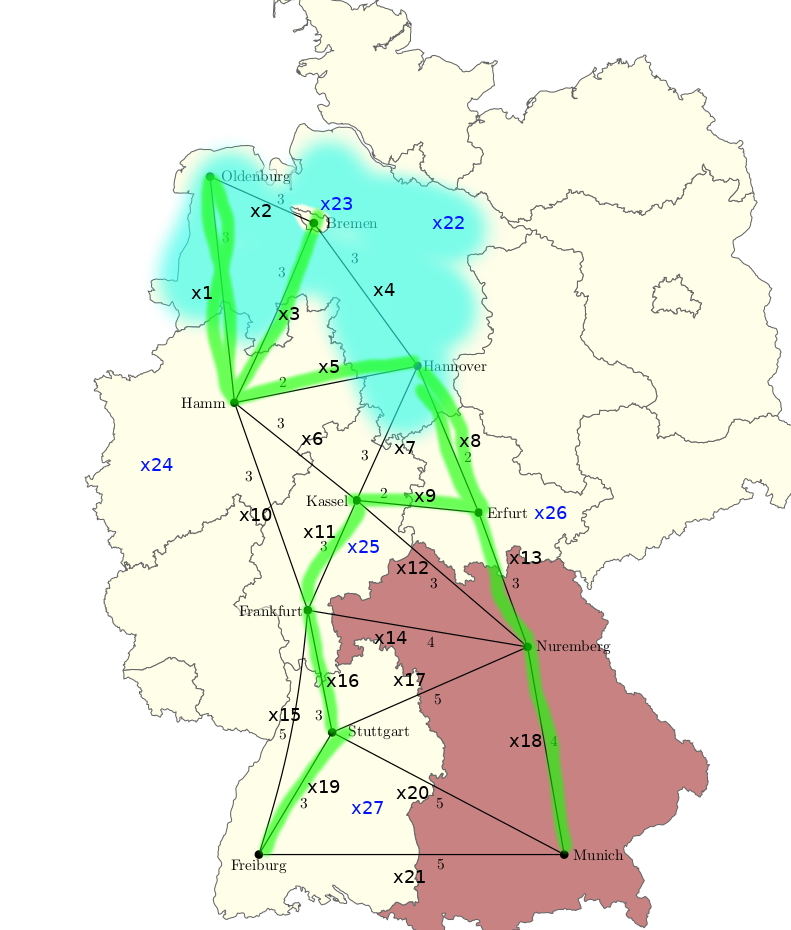
\includegraphics[scale=0.4]{de.png}
\end{center}

We introduced variables for each edge and for all states except for Bavaria because they always need an extrawurst.
The city variables are used to choose the relaxed state.
The marked edges and blue state in the image are the optimal solution we gathered with our constraints

We made some ``static'' constraints by hand and built the other constraints from the provided cuts.
All the handmade lines have a descriptive comment.
First, we want to minimize the total cost of the used edges.
Then we set the sum of all relaxed states to be smaller or equal than 1 (So there is just 0 or 1 relaxed state).

Now, for every state, we subtract the adjacent edges and require their sum to be more than $-3$ (Maximum of three connections in a state).
Bavaria is a special case which has this limit set to 2 instead of 3.
All states except for Munich also have their relaxed-state-variable included so that if it is is set, the state can have 999 extra connections. This number can also be any other number larger than the number of possible states in the state.

Lastly, we applied some replacements on the given file. Essentially we transform them, so that every cut through the graph has at least one edge connecting to the other side of the cut (sum more than 1). This causes the spanning tree that connects all cities.

The script used to replace the variables follows first. 

\lstinputlisting{replace_edges.sh}
\lstinputlisting{deutschland.opd}

\end{document}
